\chapter{Discussion et analyse critique}\label{cap:discussion}
%--------------------------------------

\section{Apports de l'approche agentique}

L'approche agentique apporte une réponse crédible à plusieurs limites des chaînes quantitatives classiques. Une stratégie multifactorielle produit souvent des sorties numériques difficiles à contextualiser : scores, expositions, contraintes actives, turnover et attribution. Les agents peuvent transformer ces sorties en une note compréhensible, relier les mouvements du portefeuille à des événements de marché et signaler les cas où le modèle statistique semble en contradiction avec l'information qualitative.

Le deuxième apport est organisationnel. Une architecture multi-agents reproduit la séparation des responsabilités d'un desk : recherche, risque, conformité, exécution et supervision. Cette séparation rend le système plus auditable qu'un agent monolithique. Elle permet aussi de tester chaque agent séparément : exactitude des synthèses pour l'agent actualités, respect des limites pour l'agent risque, complétude documentaire pour l'agent conformité.

Le troisième apport concerne la mémoire. Des projets comme FinMem montrent qu'un agent peut conserver un historique structuré des événements et de ses propres décisions. Dans un contexte de marché, cette mémoire doit être contrôlée : elle peut aider à détecter les régimes récurrents, mais elle peut aussi renforcer des biais si elle n'est pas validée par des métriques objectives.

\section{Risques spécifiques}

Les risques spécifiques sont reliés à des contrôles, à des responsables et à des décisions observables. Cette présentation évite de traiter une faiblesse agentique comme un simple problème de rédaction.

\begin{table}[H]
\centering
\caption{Risques agentiques, contrôles et responsabilités.}
\label{tab:risques-agentiques}
\scriptsize
\begin{adjustbox}{width=\textwidth}
\begin{tabular}{p{0.16\textwidth}p{0.22\textwidth}p{0.20\textwidth}p{0.27\textwidth}p{0.11\textwidth}}
\toprule
\textbf{Risque} & \textbf{Exemple} & \textbf{Conséquence} & \textbf{Contrôle} & \textbf{Responsable} \\
\midrule
Hallucination & Source inexistante ou chiffre mal interprété. & Décision fondée sur une information fausse. & Récupération sourcée, validation des citations, blocage si source invalide. & Conformité \\
Surapprentissage narratif & Explication convaincante d'un signal non robuste. & Confusion entre récit et preuve financière. & Séparation temporelle, coûts, benchmark et tests de sensibilité. & Quant et risque \\
Permission excessive & Agent autorisé à modifier les poids ou à appeler l'exécution. & Action non validée et difficile à annuler. & Permissions minimales, outils déterministes et validation humaine. & IT et risque \\
Dépendance au modèle & Réponse différente après changement de version. & Décision non reproductible ou dérive de comportement. & Versionnement des modèles, prompts, données, outils et sorties. & Propriétaire IA \\
Désaccord non traité & Agents risque et portefeuille produisent des avis incompatibles. & Consensus artificiel et perte d'un signal d'alerte. & Conservation des avis, escalade et décision humaine explicite. & Superviseur \\
\bottomrule
\end{tabular}
\end{adjustbox}
\end{table}

\section{Explicabilité : trois niveaux}

\subsection{Explicabilité quantitative}

Elle relie la décision aux rendements, aux facteurs, aux pondérations, aux coûts, aux contraintes et aux métriques de risque. Les valeurs doivent provenir des sorties du moteur déterministe et pouvoir être recalculées avec la même version de données.

\subsection{Explicabilité agentique}

Elle décrit les sources consultées, les outils appelés, l'état parcouru, les règles appliquées, le niveau de confiance et les éventuels désaccords entre agents. Une synthèse ne peut être considérée comme fiable que si ses citations et ses entrées structurées sont vérifiables.

\subsection{Explicabilité de la décision finale}

Elle identifie l'avis du superviseur, la règle ou la personne qui a validé, modifié, rejeté ou différé la recommandation. Elle précise également si une permission d'exécution existait. Le journal JSON est donc l'élément de preuve ; la note en langage naturel en est l'interface de lecture.

\begin{figure}[H]
\centering
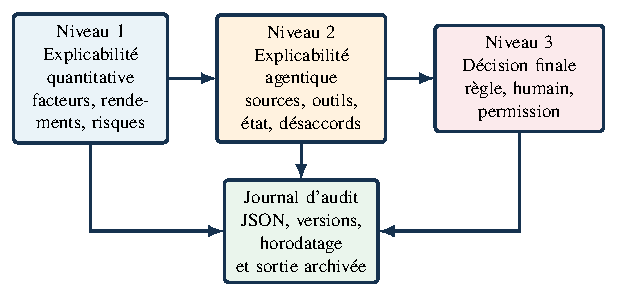
\includegraphics[width=\textwidth]{figures/schemas/explicabilite_trois_niveaux.pdf}
\caption{Trois niveaux d'explicabilité reliés au journal d'audit.}
\label{fig:explicabilite-trois-niveaux}
\end{figure}

\section{Positionnement des solutions GitHub}

Les solutions GitHub identifiées peuvent être positionnées sur une échelle de maturité.

Les frameworks comme LangGraph, AutoGen, CrewAI et Semantic Kernel sont matures pour orchestrer des workflows, mais ils ne connaissent pas le métier du trading. Ils sont adaptés à la couche agentique, pas au moteur financier.

Les plateformes comme Qlib, Lean, OpenBB, FinRL et Freqtrade sont utiles pour construire le socle quantitatif. Elles apportent données, backtesting, simulation ou environnement d'apprentissage. Elles ne garantissent pas l'explicabilité agentique, mais elles permettent de rendre les calculs reproductibles.

Les projets comme TradingAgents, FinRobot, FinMem et AI Hedge Fund sont les plus proches de l'intuition multi-agents. Leur valeur est exploratoire : ils montrent comment découper les rôles et produire des analyses financières. Leur faiblesse est le passage à l'échelle réglementaire : contrôle des données, validation indépendante, limites de risque, sécurité, audit et intégration à une infrastructure institutionnelle.

\section{Conditions minimales de mise en production}

Avant un déploiement réel, un système agentique de trading devrait satisfaire au minimum les conditions suivantes :
\begin{itemize}
    \item fonctionnement initial en mode observation, sans exécution automatique ;
    \item jeux de tests sur données historiques et scénarios extrêmes ;
    \item séparation stricte entre agents de recherche, agents de décision et outils d'exécution ;
    \item limites de risque codées hors LLM et impossibles à contourner par prompt ;
    \item registre d'audit complet et horodaté ;
    \item validation indépendante par risque, conformité et IT ;
    \item plan de repli en cas d'indisponibilité du modèle ou de dérive des sorties ;
    \item revue périodique des performances financières et des erreurs agentiques.
\end{itemize}

La trajectoire raisonnable est donc graduelle : assistant de recherche, assistant de reporting, assistant de revue de risque, puis assistant de recommandation supervisée. Le passage à une autonomie d'exécution ne devrait être envisagé qu'après une longue période de monitoring et seulement pour des stratégies à périmètre limité.

\section{Résultats du prototype expérimental}

Le prototype présenté au chapitre~\ref{cap:methodologie} fournit une première mesure du comportement d'une combinaison équipondérée de quatre sleeves factoriels. Les résultats sont comparés à l'ETF \texttt{SPY} sur la période février 2015-décembre 2025, qui correspond aux rendements mensuels calculés à partir des cours ajustés.

\begin{table}[H]
\centering
\caption{Résultats du prototype multifactoriel et du benchmark.}
\label{tab:resultats-backtest}
\scriptsize
\begin{tabular}{lrrrrrr}
\toprule
\textbf{Scénario} & \textbf{Rend. ann.} & \textbf{Vol. ann.} & \textbf{Sharpe} & \textbf{Drawdown} & \textbf{Valeur finale} & \textbf{Turnover mensuel} \cr
\midrule
SPY & 13,95\,\% & 14,96\,\% & 0,946 & -23,93\,\% & 411,73 & - \cr
Multifactoriel, 0 pb & 12,11\,\% & 14,17\,\% & 0,876 & -23,84\,\% & 345,38 & 1,26\,\% \cr
Multifactoriel, 10 pb & 12,10\,\% & 14,17\,\% & 0,875 & -23,86\,\% & 344,82 & 1,26\,\% \cr
Multifactoriel, 30 pb & 12,06\,\% & 14,17\,\% & 0,873 & -23,88\,\% & 343,69 & 1,26\,\% \cr
\bottomrule
\end{tabular}
\end{table}

Sur cette période, le benchmark \texttt{SPY} obtient le rendement annualisé le plus élevé et le meilleur ratio de Sharpe. Le portefeuille multifactoriel présente toutefois une volatilité et un drawdown légèrement inférieurs. Les coûts de transaction modifient peu le résultat dans cette configuration, car le turnover mensuel moyen reste limité.

Une vérification temporelle est également effectuée sur la période hors échantillon 2021-2025. À 10 points de base, le multifactoriel obtient un rendement annualisé de 11,45\,\%, une volatilité de 14,37\,%, un Sharpe de 0,816 et une valeur finale de 170,33. Sur la même période, SPY atteint 14,60\,%, 15,14\,%, 0,965 et 195,39. Cette comparaison confirme la prudence de l'interprétation : le prototype ne montre pas de supériorité du multifactoriel, mais fournit une base reproductible pour tester l'architecture.

\begin{table}[H]
\centering
\caption{Contrôle hors échantillon sur la période 2021-2025.}
\label{tab:resultats-oos}
\scriptsize
\begin{tabular}{lrrrrrr}
\toprule
\textbf{Scénario} & \textbf{Rend. ann.} & \textbf{Vol. ann.} & \textbf{Sharpe} & \textbf{Drawdown} & \textbf{Valeur finale} & \textbf{Turnover mensuel} \\
\midrule
SPY & 14,60\,\% & 15,14\,\% & 0,965 & -23,93\,\% & 195,39 & - \\
Multifactoriel, 10 pb & 11,45\,\% & 14,37\,\% & 0,816 & -23,86\,\% & 170,33 & 1,53\,\% \\
\bottomrule
\end{tabular}
\end{table}

\begin{figure}[H]
    \centering
    
\includegraphics[width=0.94\textwidth]{figures/cumulative_wealth.png}
    \caption{Évolution d'un investissement initial de 100 unités.}
    \label{fig:cumulative-wealth}
\end{figure}

\begin{figure}[H]
    \centering
    
\includegraphics[width=0.94\textwidth]{figures/drawdown.png}
    \caption{Drawdown du benchmark et des portefeuilles multifactoriels.}
    \label{fig:drawdown}
\end{figure}

Ces résultats ne prouvent donc pas la supériorité financière de la stratégie multifactorielle. Ils montrent plutôt l'intérêt d'un socle quantitatif reproductible auquel un agent peut être relié. L'agent pourrait recevoir ces sorties structurées afin de produire une note de décision, mais il ne doit ni recalculer les métriques ni modifier les pondérations sans règle déterministe et validation humaine.

\section{Démonstration de la couche agentique}

Le module \texttt{agent\_workflow.py} exécute désormais ce scénario avec LangGraph. Les deux exemples du 30 novembre et du 31 décembre 2025 sont générés à partir des sorties structurées du rééquilibrage, sans nouvel appel de données et sans accès aux ordres. Le premier exemple correspond au 30 novembre 2025 : les rendements de VLUE, MTUM, QUAL et USMV sont respectivement de +2,50\,\%, -1,56\,\%, +0,91\,\% et +2,31\,\%. Le rendement net du portefeuille est de +1,04\,\% pour un turnover de 1,35\,\%. La note conclut que la hausse de VLUE et USMV compense la baisse de MTUM et recommande de conserver les pondérations cibles de 25\,\%, sous réserve d'une validation humaine.

Le second exemple correspond au 31 décembre 2025 : VLUE progresse de +2,90\,\%, MTUM de +0,29\,\%, QUAL de +0,58\,\% et USMV recule de -0,82\,\%. Le rendement net du portefeuille atteint +0,74\,\% pour un turnover de 1,07\,\%. La note identifie VLUE comme principal facteur favorable, signale la contribution négative de USMV et ne propose aucun ajustement exceptionnel.

Ces notes sont comparées aux fichiers de sortie du prototype selon quatre critères : fidélité aux chiffres, complétude, respect des permissions et explicitation des limites. Le résultat est observable sur les deux exécutions ; cette évaluation manuelle constitue une première vérification qualitative et non une mesure statistique de la qualité d'un agent.

\begin{table}[H]
\centering
\caption{Évaluation des deux démonstrations agentiques.}
\label{tab:evaluation-agent}
\scriptsize
\begin{adjustbox}{width=\textwidth}
\begin{tabular}{p{0.15\textwidth}p{0.18\textwidth}p{0.18\textwidth}p{0.18\textwidth}p{0.20\textwidth}p{0.08\textwidth}}
\toprule
\textbf{Date} & \textbf{Fidélité aux chiffres} & \textbf{Complétude} & \textbf{Permissions} & \textbf{Limites explicitées} & \textbf{Résultat} \\
\midrule
30/11/2025 & Conforme : rendements, net et turnover cohérents avec le JSON. & Conforme : facteurs favorables et défavorables identifiés. & Conforme : aucun changement de poids ni ordre. & Conforme : validation humaine et limites du moteur signalées. & Conforme \\
31/12/2025 & Conforme : rendements, net et turnover cohérents avec le JSON. & Conforme : VLUE et USMV sont correctement contextualisés. & Conforme : aucun changement de poids ni ordre. & Conforme : validation humaine et limites du moteur signalées. & Conforme \\
\bottomrule
\end{tabular}
\end{adjustbox}
\end{table}

\section{Synthèse}

L'approche agentique est pertinente pour un desk multifactoriel si elle est conçue comme une architecture de coordination et d'explicabilité. Elle devient fragile si elle est présentée comme un substitut au modèle quantitatif ou au contrôle humain. Le meilleur compromis consiste à combiner des agents spécialisés avec des moteurs déterministes, des règles non contournables et un journal de décision exploitable par un auditeur.

% Texte d'exemple du template conservé hors compilation.
